\section{VNA measurements and impedance transformation discussion} 

This section details the practical experiments that were conducted with the Vector Network Analyzer (VNA) and the assembly and testing of a Radio-Frequency Front-End (RFFE) receiver. 

\subsection{Impedance transformation with an L-Match network}

The L-Match network is a simple and effective way to match a source impedance to a load impedance. In this section, the performance of an L-Match network was analyzed. The network was designed to match a source impedance of \( Z_0 = \SI{50}{\ohm} \) to a load impedance of \( Z_L = \SI{200}{\ohm} \), as shown in Figure \ref{fig:match_network}.

\begin{figure}[H]
    \centering
    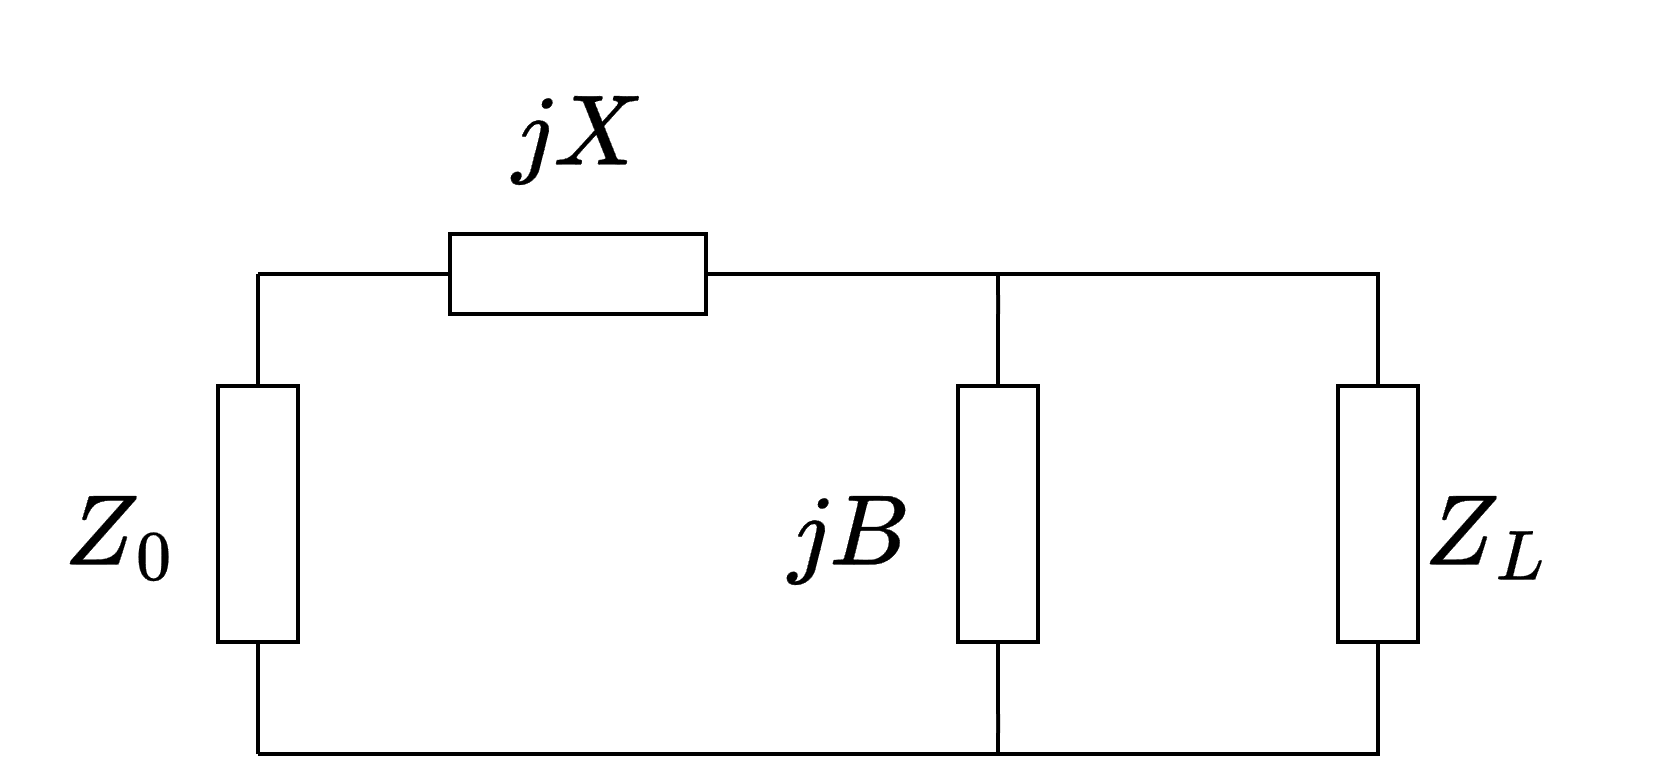
\includegraphics[width=0.5\textwidth]{Images/input-matching.png}
    \caption{L-Match Network for Impedance Transformation}
    \label{fig:match_network}
\end{figure}

\subsubsection{Theoretical Demonstration}
The L-Match network shown in Figure \ref{fig:match_network} is designed to transform a load impedance $Z_L$ into a desired input impedance $Z_{0}$. 

The total input impedance $Z_{0}$ is the sum of the series reactance $jX$ and the impedance of the parallel combination of $Z_L$ and $jB$\textsuperscript{\cite{Gillermo-Gonzalez}}:
\begin{equation}
    Z_{0} = jX + (Z_L \parallel jB)
\end{equation}

The impedance of the parallel portion ($Z_p$) is:
\begin{equation}
    Z_p = \frac{Z_L \cdot (jB)}{Z_L + jB}
\end{equation}

To simplify, this expression can be rationalized:
\begin{equation}
    Z_p = \left( \frac{jB Z_L}{Z_L + jB} \right) \cdot \left( \frac{Z_L - jB}{Z_L - jB} \right) = \frac{jB Z_L^2 + B^2 Z_L}{Z_L^2 + B^2}
\end{equation}

Separating the real ($R_p'$) and imaginary ($X_p'$) parts of $Z_p$:
\begin{equation}
    Z_p = \underbrace{\left( \frac{Z_L B^2}{Z_L^2 + B^2} \right)}_{R_p'} + j \underbrace{\left( \frac{Z_L^2 B}{Z_L^2 + B^2} \right)}_{X_p'}
\end{equation}

Now, substituting this back into the equation for $Z_{0}$:
\begin{equation}
    Z_{0} = R_p' + jX_p' + jX_A = \left( \frac{Z_L B^2}{Z_L^2 + B^2} \right) + j \left( X + \frac{Z_L^2 B}{Z_L^2 + B^2} \right)
\end{equation}

For a perfect impedance match, $Z_{0}$ must be purely resistive and equal to $R_{in}$ (e.g., \SI{50}{\ohm}). This imposes two conditions:

\begin{enumerate}
    \item \textbf{Real Part:} The real part of $Z_{0}$ must equal $R_{in}$.
    \begin{equation}
        Z_{0} = \frac{Z_L B^2}{Z_L^2 + B^2}
    \end{equation}

    \item \textbf{Imaginary Part:} The imaginary part of $Z_{0}$ must be zero.
    \begin{equation}
        X + \frac{Z_L^2 B}{Z_L^2 + B^2} = 0 \implies X= - \left( \frac{Z_L^2 B}{Z_L^2 + B^2} \right)
    \end{equation}
\end{enumerate}

These equations demonstrate that by choosing appropriate values for $X$ and $B$, the transformation is possible. Condition 2 shows that $X$ and $B$ must have opposite signs (one must be an inductor, the other a capacitor) for the reactances to cancel, leaving a purely resistive input.

\subsubsection{Design Example and Component Calculation}
The example provided in the Lab Assignment of transforming $R_L = \SI{200}{\ohm}$ to $Z_{0} = \SI{50}{\ohm}$ was used. 

\textbf{1. Calculate Required Reactances ($X$ and $B$)}

The formulas derived from the real and imaginary parts of the $Z_{0}$ equation were used, solving for $X$ and $B$ directly.

\begin{itemize}
    \item \textbf{Shunt Reactance ($B$):}
    Starting from the real part equation, it was rearranged to solve for $B^2$:
    \begin{equation}
        Z_{0} = \frac{Z_L B^2}{Z_L^2 + B^2}
    \end{equation}
    \begin{equation}
        Z_{0} (Z_L^2 + B^2) = Z_L B^2
    \end{equation}
    \begin{equation}
        Z_{0} Z_L^2 = B^2 (Z_L - Z_{0})
    \end{equation}
    \begin{equation}
        B^2 = \frac{Z_{0} Z_L^2}{Z_L - Z_{0}}
    \end{equation}
    Taking the square root for the magnitude:
    \begin{equation}
        |B| = \sqrt{\frac{\SI{50}{\ohm} \cdot (\SI{200}{\ohm})^2}{\SI{200}{\ohm} - \SI{50}{\ohm}}} = \sqrt{\frac{50 \cdot 40000}{150}} = \sqrt{\frac{2000000}{150}}
    \end{equation}
    \begin{equation}
        \mathbf{|B| \approx \SI{115.47}{\ohm}}
    \end{equation}

    \item \textbf{Series Reactance ($X$):}
    A simpler relationship can be found:
    \begin{equation}
        |X| = \sqrt{Z_{0} (Z_L - Z_{0})}
    \end{equation}
    \begin{equation}
        |X| = \sqrt{\SI{50}{\ohm} \cdot (\SI{200}{\ohm} - \SI{50}{\ohm})} = \sqrt{50 \cdot 150} = \sqrt{7500}
    \end{equation}
    \begin{equation}
        \mathbf{|X| \approx \SI{86.60}{\ohm}}
    \end{equation}
\end{itemize}

To achieve the match, the reactances must be $|X| = \SI{86.60}{\ohm}$ and $|B| = \SI{115.47}{\ohm}$.

\textbf{2. Component Value Calculation (f = 490 kHz)}
To calculate the specific inductor (L) and capacitor (C) values, the design frequency $\mathbf{f = \SI{490}{\kilo\hertz}}$ (\SI{490}{\kilo\hertz}) from the Lab Assignment was used.

The angular frequency ($\omega$) is:
\begin{equation}
    \omega = 2 \pi f = 2 \pi (\SI{490}{\kilo\hertz}) \approx \mathbf{\SI{3.0788}{§mega\radian\per\second}}
\end{equation}

\begin{itemize}
    \item \textbf{Case 1: Low-Pass Design ($X = L, B = C$)}
    \begin{itemize}
        \item \textbf{Series Inductor ($L_X$):} 
        \begin{equation}
            L_X = \frac{|X|}{\omega} = \frac{\SI{86.60}{\ohm}}{\SI{3.0788}{\mega\radian\per\second}} \approx \SI{28.127}{\micro\henry} = \mathbf{\SI{28.13}{\micro\henry}}
        \end{equation}
        \item \textbf{Shunt Capacitor ($C_B$):} 
        \begin{equation}
            C_B = \frac{1}{\omega |B|} = \frac{1}{(\SI{3.0788}{\mega\radian\per\second}) \cdot \SI{115.47}{\ohm}} \approx \SI{2.813}{\nano\farad}
        \end{equation}
    \end{itemize}

    \item \textbf{Case 2: High-Pass Design ($X = C, B = L$)}
    \begin{itemize}
        \item \textbf{Series Capacitor ($C_X$):} 
        \begin{equation}
            C_X = \frac{1}{\omega |X|} = \frac{1}{(\SI{3.0788}{\mega\radian\per\second}) \cdot \SI{86.60}{\ohm}} \approx \SI{3.751}{\nano\farad}
        \end{equation}
        \item \textbf{Shunt Inductor ($L_B$):} 
        \begin{equation}
            L_B = \frac{|B|}{\omega} = \frac{\SI{115.47}{\ohm}}{\SI{3.0788}{\mega\radian\per\second}} \approx \SI{37.505}{\micro\henry}
        \end{equation}
    \end{itemize}
\end{itemize}

For the low-pass design, the final circuit is shown in Figure \ref{fig:lmatch_lp}.

\begin{figure}[H]
    \centering
    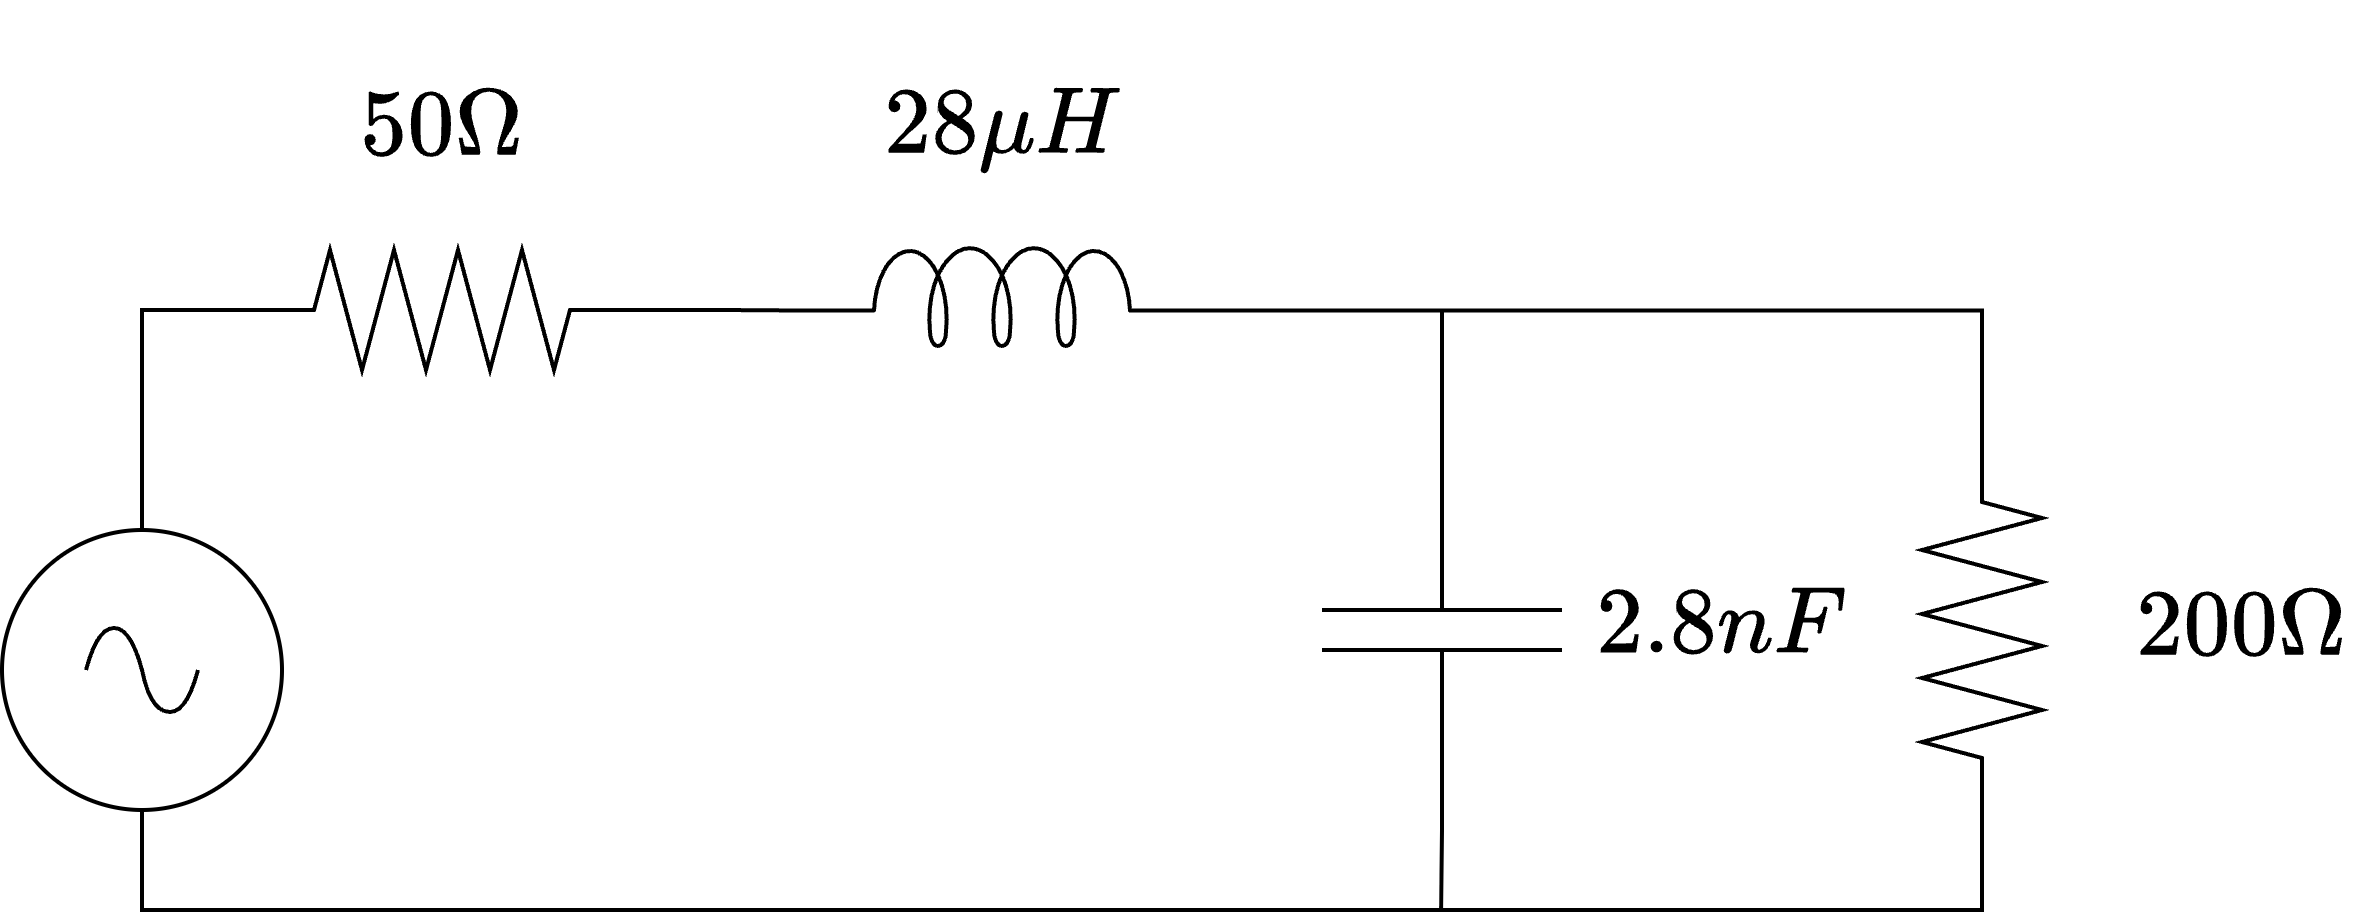
\includegraphics[width=0.6\textwidth]{Images/LC-values.png}
    \caption{Low-Pass L-Match Network Schematic}
    \label{fig:lmatch_lp}
\end{figure}

For RF applications, the low-pass configuration is often preferred due to its inherent filtering properties. In the next sections, this low-pass L-Match network was simulated and measured.

\subsubsection{Quality Factor}
The Quality Factor ($Q$) of the L-Match network is a measure of how effectively the network can perform the impedance transformation. It is defined as the ratio of the reactance to the resistance in either the series or parallel leg of the network.

The Q factor for the L-Match network can be calculated using the following equations\textsuperscript{\cite{bowick2008rf}}:

\begin{equation}
    Q = Q_s = Q_p = \sqrt{\frac{R_p}{R_s} - 1} 
\end{equation}
\begin{equation}
    Q_s = \frac{X_s}{R_s} 
\end{equation}
\begin{equation}
    Q_p = \frac{R_p}{X_p} 
\end{equation}

Where:
\begin{itemize}
    \item $Q_s = \text{the } Q \text{ of the series leg,}$
    \item $Q_p = \text{the } Q \text{ of the shunt leg,}$
    \item $R_p = \text{the shunt resistance,}$
\end{itemize}

With $R_p = \SI{200}{\ohm}$ and $R_s = \SI{50}{\ohm}$:
\begin{equation}
    Q = \sqrt{\frac{\SI{200}{\ohm}}{\SI{50}{\ohm}} - 1}
\end{equation}
\begin{equation}
    Q = \sqrt{4 - 1} = \sqrt{3}
\end{equation}
\begin{equation}
    \mathbf{Q \approx 1.732}
\end{equation}

This Q factor indicates a moderate level of selectivity and bandwidth. The higher the Q, the narrower the bandwidth.

The Q value calculated can be used to find the reactance values $X$ and $B$ to confirm the earlier calculations, where $X_s = X_A$ and $R_s = R_{in} = \SI{50}{\ohm}$:

\begin{equation}
    Q_s = \frac{X_s}{R_s}
\end{equation}
\begin{equation}
    |X| = Q_s \cdot R_s
\end{equation}
\begin{equation}
    |X| = 1.732 \cdot \SI{50}{\ohm}
\end{equation}
\begin{equation}
    \mathbf{|X| \approx \SI{86.60}{\ohm}}
\end{equation}

\begin{equation}
    Q_p = \frac{R_p}{X_p}
\end{equation}
\begin{equation}
    |B| = \frac{R_p}{Q_p}
\end{equation}
\begin{equation}
    |B| = \frac{\SI{200}{\ohm}}{1.732}
\end{equation}
\begin{equation}
    \mathbf{|B| \approx \SI{115.47}{\ohm}}
\end{equation}

These are the exact same reactance values that were calculated before, confirming the consistency of this design approach.

\subsection{Simulation in Qucs-s}

\subsubsection{Circuit schematic}
The designed L-Match network was simulated in Qucs-s to validate the theoretical calculations. The schematic of the circuit is shown in Figure \ref{fig:qucs_lmatch}.

\begin{figure}[H]
    \centering
    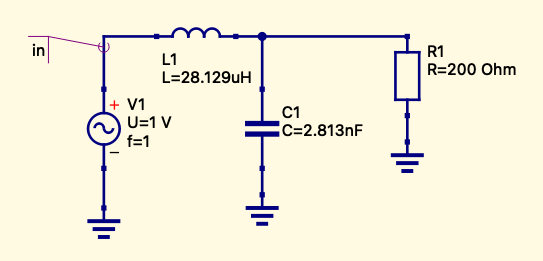
\includegraphics[width=0.5\textwidth]{Images/Qucs_LMatch.png}
    \caption{L-Match Network Schematic in Qucs-s}
    \label{fig:qucs_lmatch}
\end{figure}

\subsubsection{Input Impedance Simulation}
The input impedance ($Z_{in}$) of the L-Match network was simulated in Qucs-s to verify the theoretical calculations. The results are shown in Figure \ref{fig:qucs_zin}.

\begin{figure}[H]
    \centering
    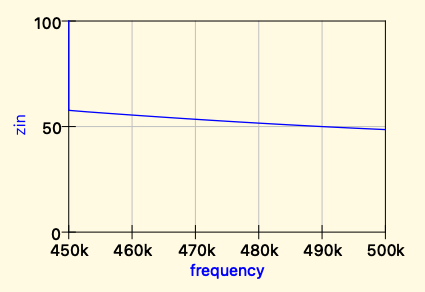
\includegraphics[width=0.5\textwidth]{Images/Qucs_Zin.png}
    \caption{Input Impedance ($Z_{in}$) of the L-Match Network in Qucs-s}
    \label{fig:qucs_zin}
\end{figure}

The simulation results confirmed that the input impedance of the L-Match network is approximately \SI{50}{\ohm} at the design frequency of \SI{490}{\kilo\hertz}, validating the theoretical calculations.

\subsubsection{Input Reflection Coefficient simulation}

The input reflection coefficient ($S_{11}$) was also simulated in Qucs-s. The results are shown in Figure \ref{fig:qucs_s11}.

\begin{figure}[H]
    \centering
    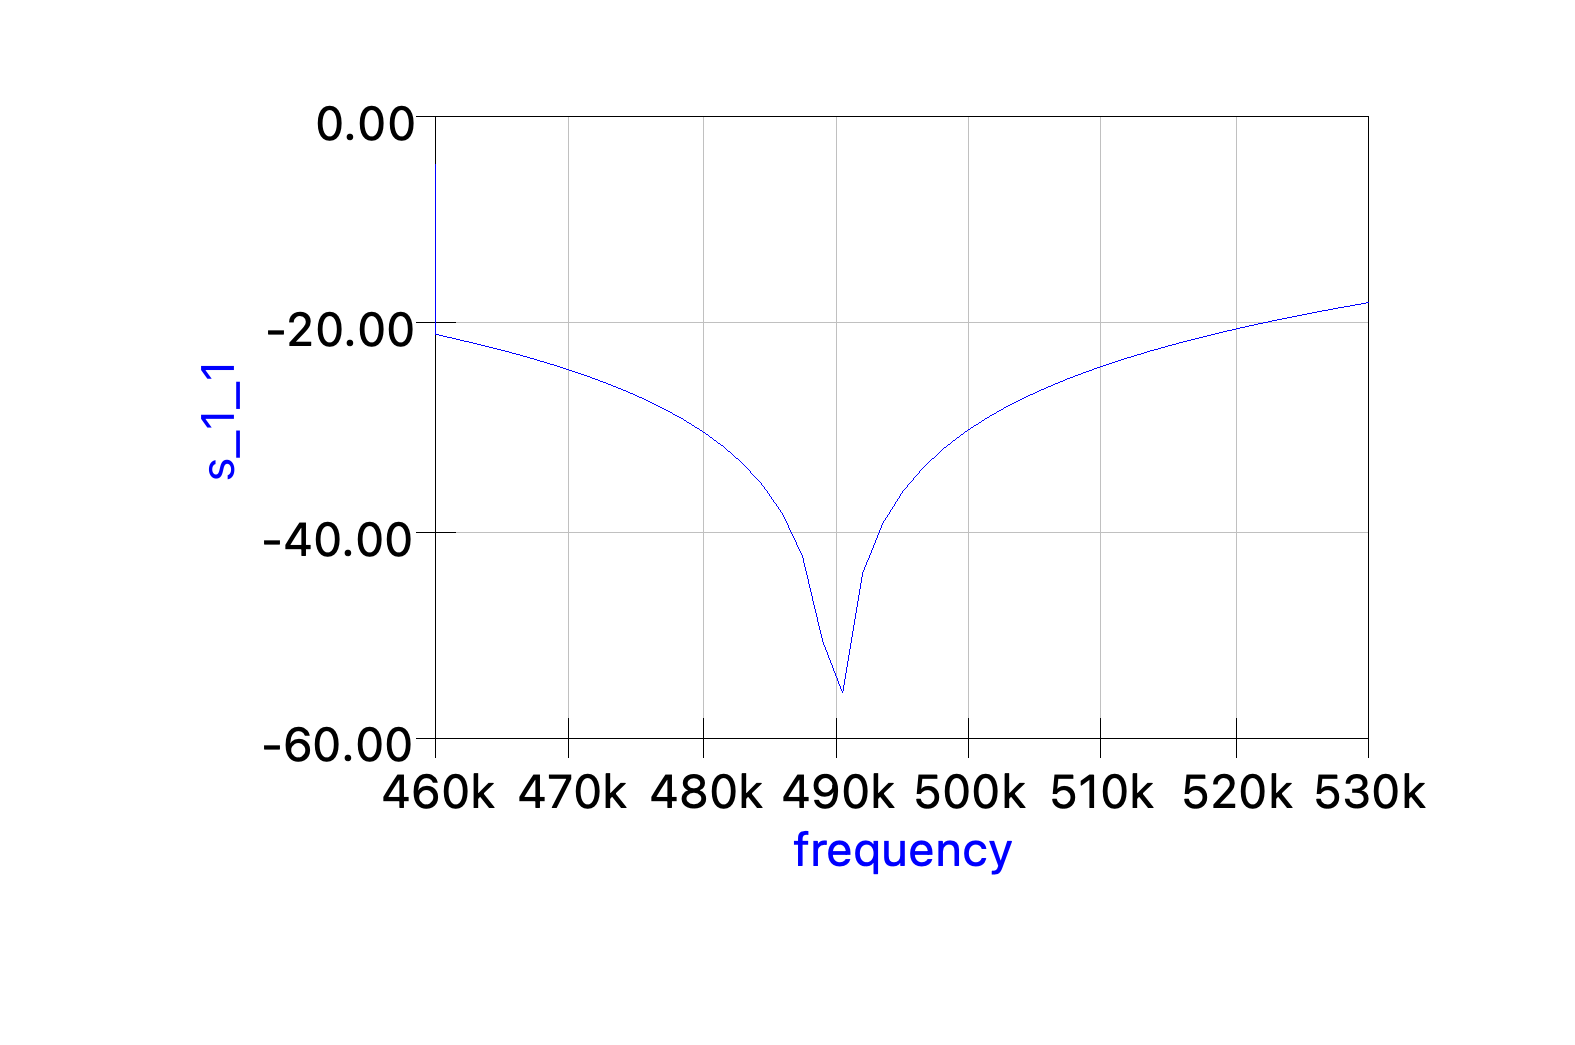
\includegraphics[width=0.5\textwidth]{Images/Qucs_S11.png}
    \caption{Input Reflection Coefficient ($S_{11}$) of the L-Match Network in Qucs-s}
    \label{fig:qucs_s11}
\end{figure}

The simulation results showed that the reflection coefficient \( S_{11} \) was minimized to approximately \SI{-58}{\deci\bel} at the design frequency of \SI{490}{\kilo\hertz}, indicating a good impedance match and demonstrating the effectiveness of the network.

\subsection{VNA Measurements and Comparison}
\label{sec:vna}

In this section, the experimental results from the L-Match network, measured with a Vector Network Analyzer (VNA), are presented and compared against the theoretical and simulated results.

\subsubsection{NanoVNA Measurement}

The assembled L-Match circuit shown in Figure \ref{fig:qucs_lmatch} was tested with a NanoVNA. The result, shown in Figure \ref{fig:nanovna}, confirmed a successful impedance match, with a measured $S_{11}$ of $\mathbf{\SI{-38.50}{\deci\bel}}$ at a frequency of $\mathbf{\SI{490.167}{\kilo\hertz}}$.

\begin{figure}[H]
    \centering
    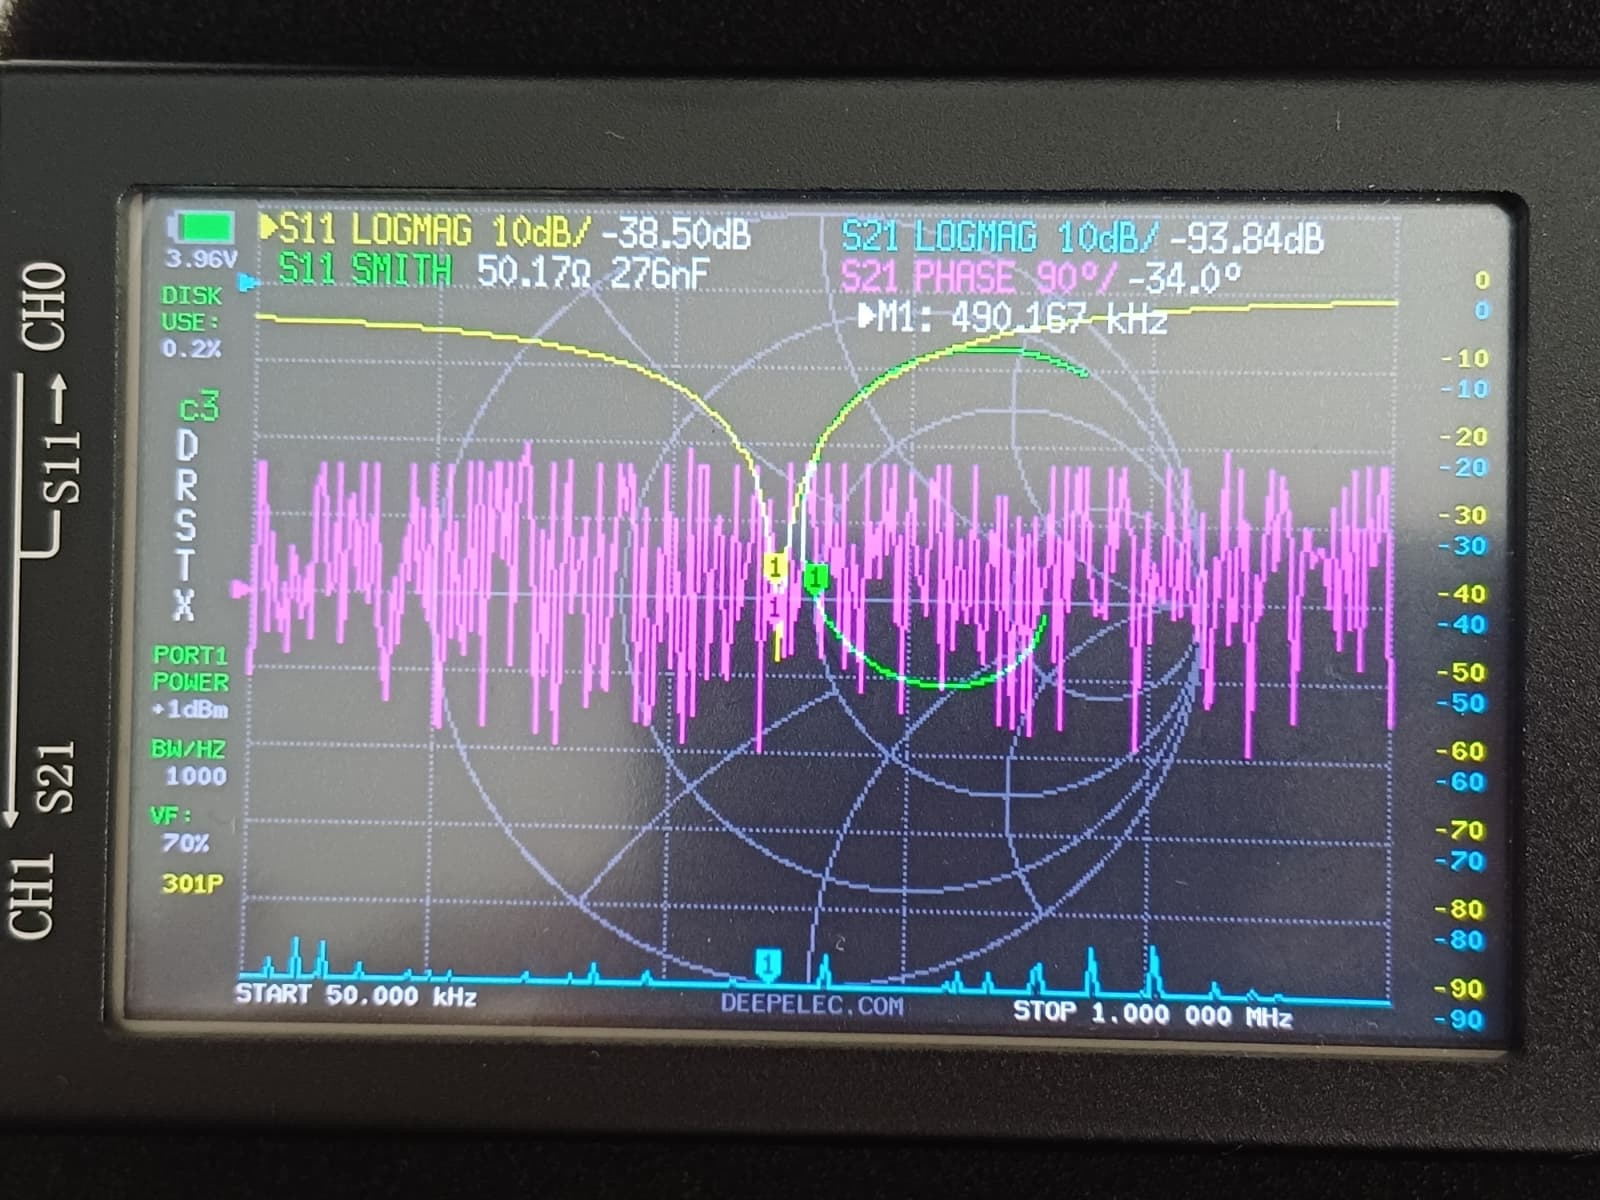
\includegraphics[width=0.5\textwidth]{Images/nanovna_s11.jpeg}
    \caption{Initial verification measurement using the calibrated NanoVNA. The marker shows a successful match of \SI{-38.50}{\deci\bel} at \SI{490.167}{\kilo\hertz}.}
    \label{fig:nanovna}
\end{figure}

\subsubsection{Secondary Verification (HP VNA)}
Following the successful initial test, the circuit was then measured on a high-precision HP 8753ES VNA to obtain a more detailed characterization. The results from this measurement are shown in Figures \ref{fig:vna_logmag} and \ref{fig:vna_smith}.

The HP VNA measurement (Figure \ref{fig:vna_logmag}) identified the point of maximum match with higher resolution:
\begin{itemize}
    \item \textbf{Minimum $S_{11}$ Frequency:} \SI{490.847}{\kilo\hertz}
    \item \textbf{Minimum $S_{11}$ Value:} \SI{-46.652}{\deci\bel}
\end{itemize}

\begin{figure}[H]
    \centering
    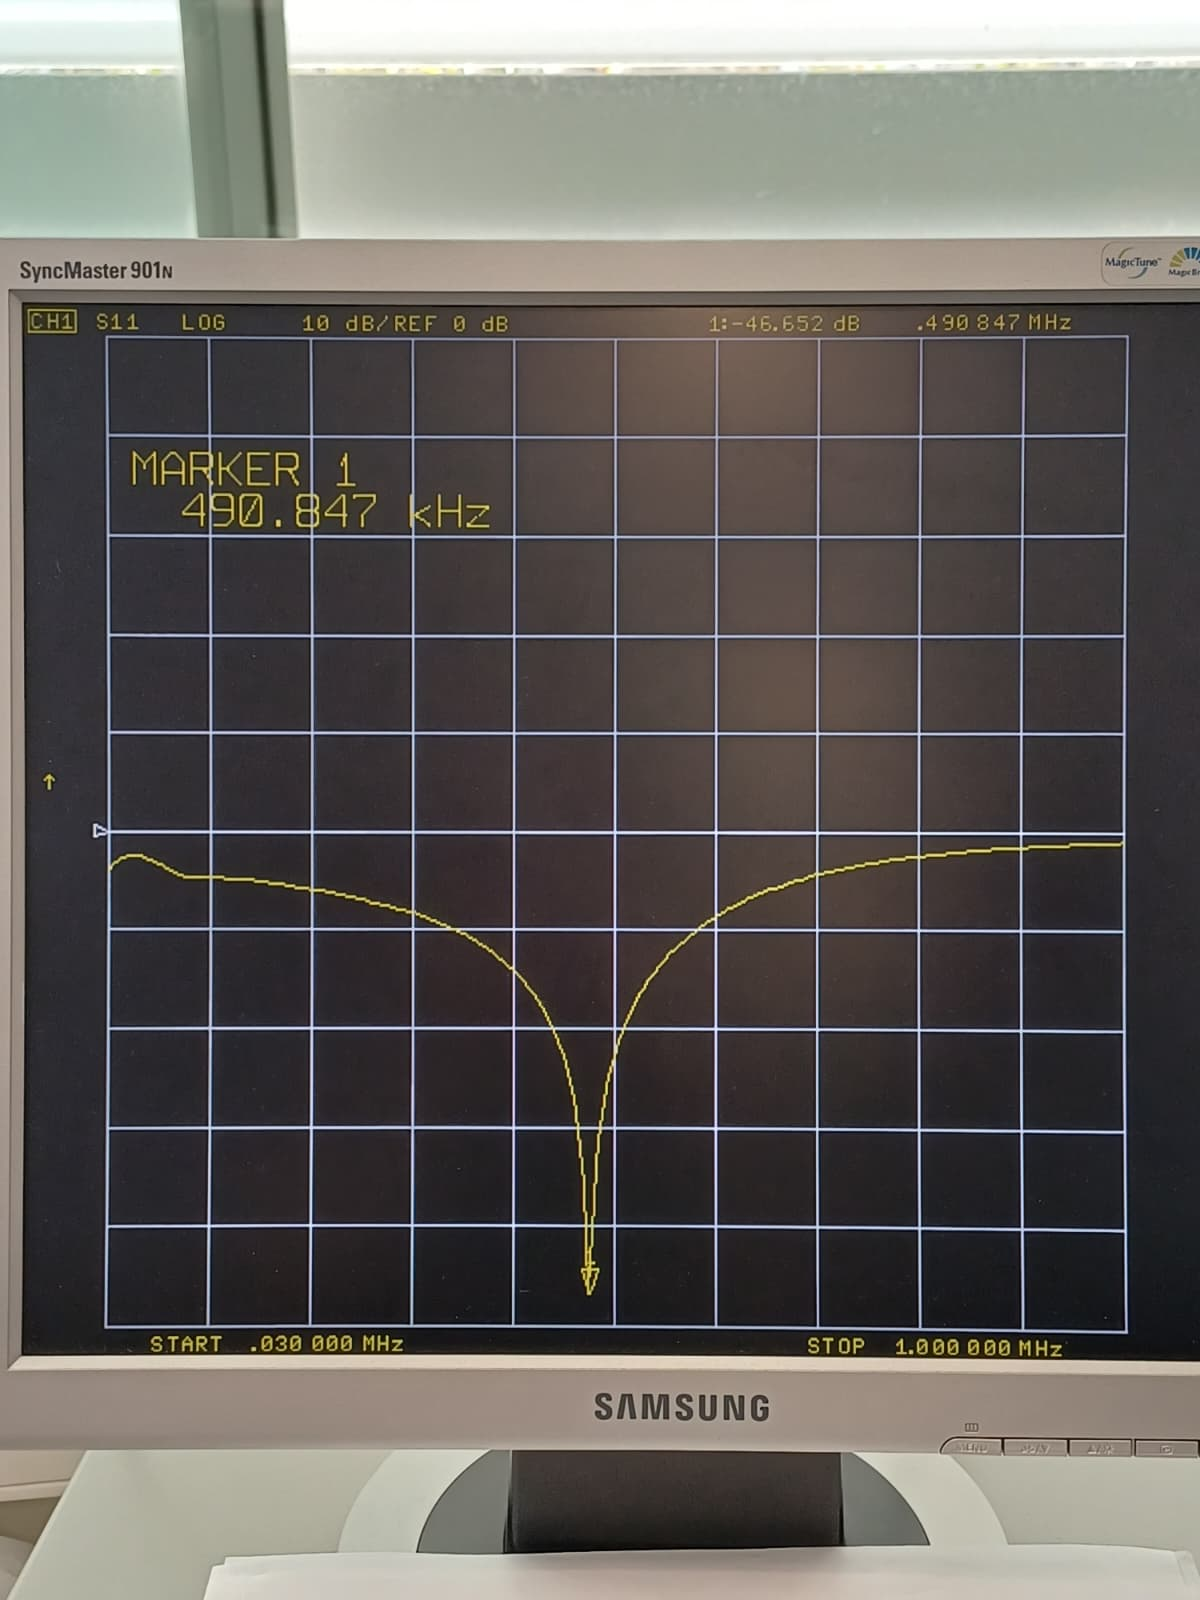
\includegraphics[width=0.4\textwidth]{Images/vna_s11_logmag.jpeg}
    \caption{High-precision VNA (HP 8753ES) measurement of $S_{11}$ (Log-Mag, dB). The marker shows a minimum of \SI{-46.652}{\deci\bel} at \SI{490.847}{\kilo\hertz}.}
    \label{fig:vna_logmag}
\end{figure}

The Smith Chart for this measurement (Figure \ref{fig:vna_smith}) confirmed this result, showing the marker positioned almost perfectly at the center of the chart ($1+j0$).

\begin{figure}[H]
    \centering
    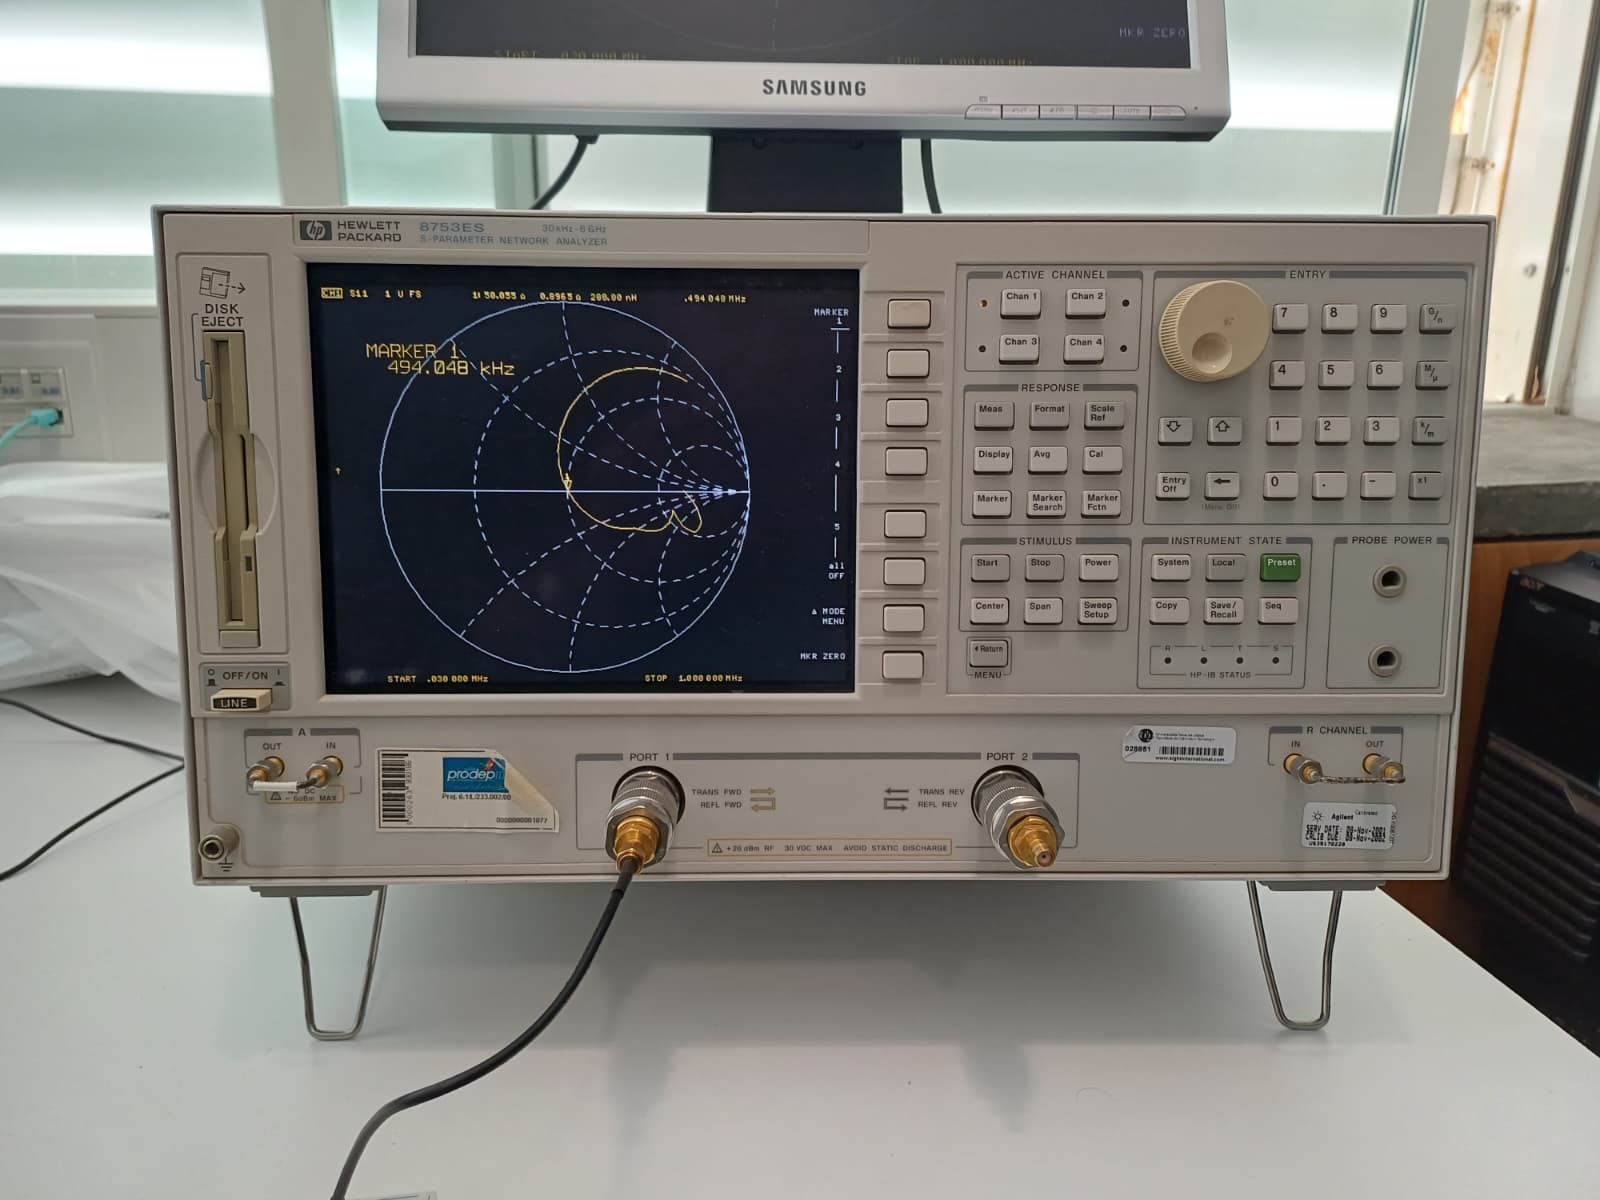
\includegraphics[width=0.6\textwidth]{Images/vna_s11_smith.jpeg}
    \caption{HP VNA measurement of $S_{11}$ (Smith Chart). The marker confirms the match at the center (\SI{50}{\ohm}).}
    \label{fig:vna_smith}
\end{figure}


\subsubsection{Comparison and Analysis}
To evaluate the success of the design, the results from all three methods are compared. The more precise data from the HP VNA was used for the final comparison.

\begin{table}[H]
    \centering
    \caption{Comparison of Theoretical, Simulated, and Experimental Results.}
    \label{tab:comparison}
    \begin{tabularx}{\textwidth}{ >{\centering\arraybackslash}X
                                  >{\centering\arraybackslash}X
                                  >{\centering\arraybackslash}X }
        \toprule
        \textbf{Method} & \textbf{Min. $S_{11}$ Frequency} & \textbf{Min. $S_{11}$ Value (dB)} \\
        \midrule
        Theoretical     & \SI{490}{\kilo\hertz}             & $-\infty$ (ideal)      \\
        \midrule
        Simulated       & \SI{490}{\kilo\hertz}             & \SI{-58}{\deci\bel}      \\
        \midrule
        \textbf{Measured (HP VNA)} & $\mathbf{\SI{490.847}{\kilo\hertz}}$ & $\mathbf{\SI{-46.652}{\deci\bel}}$     \\
        \bottomrule
    \end{tabularx}
\end{table}

\textbf{Analysis:}
\begin{itemize}
    \item \textbf{Frequency:} The experimental result (\SI{490.847}{\kilo\hertz}) was exceptionally close to the theoretical target (\SI{490}{\kilo\hertz}), with an error of only \SI{0.17}{\percent}. This minor deviation was likely due to the standard manufacturing tolerances of the physical components used.
    
    \item \textbf{$S_{11}$ Value:} The measured value of \SI{-46.652}{\deci\bel} was an excellent result. It indicated that only \SI{0.0002}{\percent} of the signal power was reflected. The fact this value was not infinite (like theory) or as low as the ideal simulation was due to the non-ideal nature of the components. 
\end{itemize}

\textbf{Conclusion:} The experimental measurements, first verified with the NanoVNA and then characterized with the HP VNA, successfully validated the theoretical design. The L-Match circuit demonstrated a successful impedance match at the target frequency.